\documentclass[11pt,a4paper,oneside]{scrartcl}

\usepackage[utf8]{inputenc}
\usepackage[ngerman]{babel}
\usepackage{amsmath, amssymb, amsthm} 
\usepackage{graphicx, tikz} 
\usepackage{hyperref} 
\usepackage{tabularx}
\usepackage[linesnumbered,ruled,vlined]{algorithm2e}

\newtheorem{satz}{Satz}[section]
\newtheorem{lemma}[satz]{Lemma}
\newtheorem{proposition}[satz]{Proposition}
\newtheorem{definition}[satz]{Definition}
\newtheorem{bemerkung}[satz]{Bemerkung}

\begin{document}

\title{Ausarbeitung zum Thema AdaBoost}
\subtitle{Bachelor-Seminar "`Top 10 Algorithms in Data Mining"'}

\author{Marius Graf}
\date{\today}

\maketitle

\tableofcontents

\begin{abstract}
    \noindent\textbf{Abstract:}
    Fassen Sie hier den Inhalt ihrer Ausarbeitung kurz zusammen.
\end{abstract}

\section{Einleitung}
Data Mining analysiert große Datenmengen, um Muster und Zusammenhänge zu erkennen,
wobei Methoden aus Statistik, Machine Learning und Datenbanktechnologie eingesetzt werden.
Es spielt eine zentrale Rolle in Forschung und Industrie, um Erkenntnisse zu gewinnen und
Entscheidungen zu unterstützen. AdaBoost, eine Methode des Data Mining, gehört zu den
Ensemble-Methoden, die mehrere Modelle kombinieren, um präzisere Vorhersagen zu treffen.
Diese Arbeit konzentriert sich auf AdaBoost, der Beobachtungen gewichtet, um schwierig zu
klassifizierende Datenpunkte besser vorherzusagen.

\section{Grundlagen des Boosting}
Boosting ist eine Ensemble-Technik im Machine Learning, die mehrere "schwache Lerner" kombiniert,
um ein präzises Gesamtmodell zu erstellen. In jeder Iteration wird ein Modell trainiert, das falsche
Vorhersagen der vorherigen Modelle korrigiert, indem es die Gewichtung der Trainingsdaten anpasst.
Das Ziel ist es, den systematischen Fehler (Bias) des Modells zu reduzieren und die Genauigkeit
schrittweise zu verbessern, indem es sich auf schwierig zu klassifizierende Datenpunkte konzentriert.

\begin{figure}[h]
    \centering
    \includegraphics[width=0.8\textwidth]{"./figures/Boosting_Graph"}
    \caption{Flussdiagramm zur Veranschaulichung des Boosting-Konzepts}
\end{figure}

\subsection*{Beispiel:}
Stellen Sie sich vor, Sie möchten ein Modell entwickeln, das den Preis von
Häusern basierend auf verschiedenen Merkmalen wie Größe, Lage, Anzahl der
Zimmer und Baujahr vorhersagt.

\begin{table}[h]
    \centering
    \begin{tabularx}{\textwidth}{|X|X|X|X|}
        \hline
        \textbf{Haus} & \textbf{Größe (in Quadratmetern)} & \textbf{Lage}    & \textbf{Preis} \\
        \hline
        Haus 1        & 100                               & Stadtzentrum     & 500.000€       \\
        \hline
        Haus 2        & 150                               & Vorort           & 300.000€       \\
        \hline
        Haus 3        & 80                                & Stadtzentrum     & 400.000€       \\
        \hline
        Haus 4        & 120                               & Ländliche Gegend & 200.000€       \\
        \hline
    \end{tabularx}
    \caption{Beispielhafte Daten für Hauspreise basierend auf Größe und Lage}
\end{table}

\begin{itemize}
    \item Sie entscheiden sich zunächst für ein sehr einfaches Modell,
          das den Preis nur anhand der Größe des Hauses vorhersagt.
          Dieses Modell geht davon aus, dass alle anderen Merkmale keinen
          Einfluss auf den Preis haben.
    \item In Wirklichkeit variieren die Hauspreise jedoch nicht nur aufgrund
          ihrer Größe, sondern auch aufgrund anderer Faktoren. Ein kleines Haus in einer
          begehrten Lage könnte teurer sein als ein großes Haus in einer weniger beliebten
          Gegend.
    \item Da Ihr Modell nur die Größe berücksichtigt und alle anderen Faktoren ignoriert,
          wird es systematisch den Preis von Häusern in begehrten Lagen unterschätzen und den Preis
          von Häusern in weniger beliebten Gegenden überschätzen. Dieser systematische Fehler in den
          Vorhersagen ist der \textbf{Bias}.
\end{itemize}

In mehreren Iterationen wird beim Boosting nun das Gewicht der Datenpunkte so angepasst, dass sich das
zweite Modell auf genau die Datenpunke fokussiert, welche zuvor besonders schlecht vorhergesagt wurden.
Somit ist hier eine deutlich größere Anpassung der Vorhersage zu erkennen als bei den Datenpunkten, die zuvor
relativ gut vorhergasagt wurden.

\begin{table}[h]
    \centering
    \begin{tabularx}{\textwidth}{|X|X|X|X|X|X|}
        \hline
        \textbf{Haus} & \textbf{Größe (in Quadratmetern)} & \textbf{Lage}    & \textbf{Tatsächlicher Preis} & \textbf{Vorhersage (Iteration 1)} & \textbf{Vorhersage (Iteration 2)} \\
        \hline
        Haus 1        & 100                               & Stadtzentrum     & 500.000€                     & 450.000€                          & 490.000€                          \\
        \hline
        Haus 2        & 150                               & Vorort           & 300.000€                     & 350.000€                          & 310.000€                          \\
        \hline
        Haus 3        & 80                                & Stadtzentrum     & 400.000€                     & 380.000€                          & 405.000€                          \\
        \hline
        Haus 4        & 120                               & Ländliche Gegend & 200.000€                     & 250.000€                          & 210.000€                          \\
        \hline
    \end{tabularx}
    \caption{Beispielhafte Daten für Hauspreise und wie Boosting den Bias in mehreren Iterationen reduziert}
\end{table}

\section{Der AdaBoost Algorithmus}
\subsection*{Einführung}
AdaBoost, ein Akronym für \glqq Adaptive Boosting\grqq. Der Algorithmus wurde in den 1990er Jahren von
den Forschern Yoav Freund und Robert Schapire entwickelt, stellt einen Meilenstein in der Geschichte
des maschinellen Lernens dar und hat die Landschaft der Ensemble-Methoden maßgeblich geprägt.
Der AdaBoost-Algorithmus unterscheidet sich von anderen Boosting-Methoden durch seine adaptiven Lernansatz.
In jeder Iteration des Trainingsprozesses passt AdaBoost die Gewichtung der Trainingsdaten basierend auf den
Fehlern der vorherigen Modelle an. Dieser iterative und adaptive Ansatz ermöglicht es dem Algorithmus,
kontinuierlich zu lernen und seine Vorhersagegenauigkeit zu verbessern.
Historisch gesehen hat die Einführung von AdaBoost den Weg für viele Weiterentwicklungen im Bereich des
Boostings geebnet. Es hat nicht nur die Effizienz und Wirksamkeit von Boosting-Methoden demonstriert,
sondern auch die Forschung in diesem Bereich vorangetrieben und zu zahlreichen Variationen und
Weiterentwicklungen geführt. \cite{WuKumar2009}

\subsection*{Notation}
\begin{itemize}
    \item
          Sei $\mathcal{X}$ die Menge der Features und $\mathcal{Y}$ die Menge der Labels, die gelernt werden sollen.
          Dabei ist $\mathcal{Y}=\{-1, +1\}$ bei binärer Klassifikation. Ein Trainingdatensatz $D$ besteht aus $m$ Einträgen,
          welche Features mit Labels verbinden:
          $$
              D=\{(\boldsymbol{x}_i, y_i)\},~i\in\{1, .., n\}
          $$
    \item Nach dem Training auf $D$ wird ein Lernalgorithmus $\mathcal{L}$ eine Hypothese bzw. einen Klassifizierer
          $h$ zurück geben, der von $\mathcal{X}$ nach $\mathcal{Y}$ abbildet.
          \begin{align*}
              h:\mathcal{X} \rightarrow \mathcal{Y} \\
              h(\boldsymbol{x}) = y
          \end{align*}
    \item $T$ ist die Anzahl der gewünschten Trainingsschleifen.
    \item Bei jeder Iteration $t\in\{1, .., T\}$ wird ein Datensatz $\mathcal{D}_t$ von $D$ abgeleitet. Dabei wird
          jeder Datenpunkt mit einem Gewicht $\mathcal{D}_t(i)$ mit $i\in\{1, ..., n\}$ erweitert.
\end{itemize}

\subsection*{Initialisierung der Gewichte}
Zu Beginn sind die Gewichte aller $n$ Datenpunkte gleich verteilt:

$$
    \mathcal{D}_1(i) = \frac{1}{n}
$$

Zudem ist die Summe aller Gewichte bei jeder Iteration stets $1$.

$$
    \sum_{i=1}^n \mathcal{D}_t(i) = 1
$$

\subsection*{Training der schwachen Lerner}
Trainiere für $t=1$ bis $T$ schwache Lerner unter berücksichtigung der aktuellen Gewichtung.

$$
    h_t = \mathcal{L}(D, \mathcal{D}_t)
$$

(Hinweis: Abhängig vom konkreten Lernalgorithmus wird ggf. zusätzlich zum gewichteten Datensatz $\mathcal{D}_t$
auch der gesamte Datensatz $D$ benötigt. Daher werden formal beide übegeben.)\\
Das Ziel ist es, den gewichteten Fehler zu minimieren:

$$
    \varepsilon_t = \sum_{i=1}^n {D}_t(i) I\left(y_i \neq h_t\left(\boldsymbol{x}_i\right)\right)
$$

$I$ ist die Indikatorfunktion, die $1$ zurückgibt, wenn $y_i\neq h_t(\boldsymbol{x_i})$ erfüllt ist, und
sonst $0$. Das bedeutet, sie gibt $1$ für jeden falsch vorhergesagten Datenpunkt zurück. $\varepsilon_t$
stellt die gewichtete Summe aller falschen Vorhersagen des $t$-ten Klassifizierers dar. Der Klassifizierer
mit dem geringsten Fehler wird in jeder Iteration ausgewählt. Ein Fehler von $1$ zeigt, dass alle
Vorhersagen falsch waren, während $0$ bedeutet, dass alle korrekt waren. Bei einem Fehler von $0.5$
waren die Hälfte der Vorhersagen richtig. Wenn $\varepsilon_t > 0.5$, sind die Vorhersagen schlechter
als zufälliges Raten, und der Algorithmus wird gestoppt, da weitere Lerner das Modell nicht verbessern würden.
\subsection*{Berechnung des Lernkoeffizienten}
Der Koeffizient $\alpha_t$ für den ausgewählen schwachen Lerner $h_t$ wird wie folgt berechnet:
$$
    \alpha_t = \frac{1}{2}\ln\left(\frac{1-\varepsilon_t}{\varepsilon_t}\right)
$$
zient gibt an, wie viel stark die Vorhersage dieses schwachen Lerners im späteren Ensemble
gewichtet wird.
\subsection*{Aktualisierung der Gewichte}
Die Gewichte der Trainingsdaten werden basierend auf den Vorhersagen des zuvor bestimmten $h_t$ aktualisiert:
\begin{align*}
    \mathcal{D}_{t+1}(i) = & \mathcal{D}_{t}(i) \times e^{-\alpha_t} & \text{ für korrekt klassifizierte Datenpunke} \\
    \mathcal{D}_{t+1}(i) = & \mathcal{D}_{t}(i) \times e^{\alpha_t}  & \text{ für falsch klassifizierte Datenpunke}
\end{align*}
Dabei werden alle neuen Gewichte zuletzt normalisiert, damit ihre Summe nach der Aktualisierung wieder $1$ ist.
\begin{align*}
    Z_t                  & =\sum_{j=1}^n\mathcal{D}_{t+1}(j)~(\text{Normalisierungsfaktor}) \\
    \mathcal{D}_{t+1}(i) & = \frac{\mathcal{D}_{t+1}(i)}{Z_t}
\end{align*}
\subsection*{Das Ergebnis des Algorithmus}
Der Algorithmus gibt ein Gesamtmodell zurück, welches die Klassifizierung des Datenpunktes durch die gewichtete
Summe aller schwachen Lerner darstellt:
\begin{align}
    H    & :      \mathcal{X} \rightarrow \{-1, +1\}      \\
    H(x) & =  sign\left(\sum_{t=1}^T\alpha_th_t(x)\right)
\end{align}
\begin{algorithm}
    \DontPrintSemicolon
    \KwData{Trainingsdatensatz $D$, wobei $x_i \in \mathcal{X}$ und $y_i \in \{-1, 1\}$; Anzahl der Iterationen $T$.}
    \KwResult{Finale Klassifikationsfunktion: $H(x) = \text{sign}\left(\sum_{t=1}^{T} \alpha_t h_t(x)\right)$.}
    \BlankLine
    \tcp{Initialisiere Gewichte}
    $\mathcal{D}_1(i)=\frac{1}{n}$\;
    \For{$t = 1$ \KwTo $T$}{
        \tcp{Trainiere einen schwachen Lerner unter Berücksichtigung der Gewichtung $\mathcal{D}_t(i)$}
        $h_t \leftarrow \mathcal{L}(D, \mathcal{D}_t)$ \;\;
        \tcp{Berechne den gewichteten Fehler}
        $\epsilon_t = \sum_{i=1}^{n} \mathcal{D}_t(i) I(y_i \neq h_t(x_i))$\;\;
        Wähle den Lerner mit dem geringsten Fehler als $h_t$\;\;
        \If{$\varepsilon_t > 0.5$}{\textbf{break}}\;
        \tcp{Berechne den Lernerkoeffizienten}
        $\alpha_t = \frac{1}{2} \ln \left( \frac{1 - \epsilon_t}{\epsilon_t} \right)$\;\;
        \tcp{Aktualisiere die Gewichte}
        \For{$i = 1$ \KwTo $n$}{
            \eIf{$y_i = h_t(x_i)$}{
                $\mathcal{D}_{t+1}(i) \leftarrow \mathcal{D}_{t}(i) \times e^{-\alpha_t}$\;
            }{
                $\mathcal{D}_{t+1}(i) \leftarrow \mathcal{D}_{t}(i) \times e^{\alpha_t}$\;
            }
        }\;
        \tcp{Normalisiere Gewichte}
        $Z_t \leftarrow \sum_{j=1}^n\mathcal{D}_{t+1}(j)$\;
        \For{$i = 1$ \KwTo $n$}{
            $\mathcal{D}_{t+1}(i) \leftarrow \frac{\mathcal{D}_{t+1}(i)}{Z_t}$\;
        }
    }
    \KwOut{$H(x)=sign\left(\sum_{t=1}^T\alpha_th_t(x)\right)$}
    \caption{AdaBoost}
\end{algorithm}
\newpage
\section{Praktische Anwendung und Beispiele}
Vor allem wegen seiner Effizienz und Genauigkeit hat sich  in einer Vielzahl
von Anwendungen bewährt. Zudem ist AdaBoost einfach zu
implementieren, hat wenige Hyperparameter und liefert oft selbst bei unvollständigen
oder verrauschten Daten.
\subsection*{Bilderkennung und Computervision}
AdaBoost wird häufig in der Gesichtserkennungstechnologie eingesetzt.
Zum Beispiel nutzen soziale Medien wie Facebook AdaBoost-Algorithmen,
um Benutzer in Fotos automatisch zu markieren. \cite{viola2001rapid}
\begin{figure*}
    \centering
    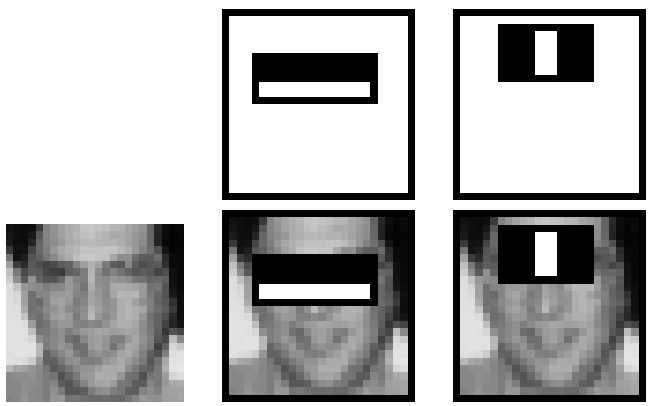
\includegraphics[width=.65\textwidth]{figures/CV_Example.png}
    \caption{Anwendung von AdaBoost bei Computer Vision:
        Das erste Merkmal von AdaBoost misst den Intensitätsunterschied
        zwischen der Augenregion und den oberen Wangen,
        wobei die Augen oft dunkler sind. Das zweite Merkmal vergleicht die
        Intensität der Augen mit der Nasenbrücke.\cite{viola2001rapid}}
\end{figure*}
\subsection*{Textklassifikation und Natural Language Processing}
E-Mail-Dienste verwenden AdaBoost, um Spam-E-Mails zu identifizieren und zu filtern.\\
\cite{panwar2022detection}
\subsection*{Medizinische Diagnostik}
AdaBoost wird in der medizinischen Forschung eingesetzt,
um das Risiko von Herzkrankheiten basierend auf Patientendaten vorherzusagen.
\subsection*{Finanzwesen}
AdaBoost wird auch im Finanzsektor eingesetzt,
um Aktienkursbewegungen vorherzusagen.
\section{Vor- und Nachteile von AdaBoost}
Zu den Vorteilen von AdaBoost zählen vor allem seine Einfachheit. AdaBoost ist simpel zu
implementieren und erfordert in der Regel nur geringe bis keine Anpassung des Lernalgorithmus,
wodurch eine Vielseitigkeit gegeben ist, da pronzipiell jeder Klassifizierungsalgorithmus
als Basislerner dienen kann.
Zudem ist AdaBoost aufgrund seiner schwachen Lerner weniger anfällig für Overfitting und Adaboost
kann automatisch wichtige Features identifizieren, was besonders nützlich ist, wenn viele
Features vorhanden sind.\\\\
Die Nachteile von AdaBoost sind, dass es empfindlicher gegenüber verrauschten Daten und Außreißer
ist, da AdaBoost versucht, jeden Datenpunkt korrekt zu klassifizieren. Zudem kann AdaBoost bei
großen Datensätzen zeitaufwändig sein und erheblichen Speicherplatz benötigen. Letztlich
ist AdaBoost vor allem Stark von seinem Basislerner abhängig und von Natur aus nur für
binäre Klassifikation konzentriert.
\section{Erweiterungen und Variationen von AdaBoost}
AdaBoost wurde ursprünglich für binäre Klassifikation entwickelt. Mit Erweiterungen und
Variationen ist der Algorithms jedoch in der Lage, auch auf andere Arten von Problemen
angewandt zu werden.

\begin{itemize}
    \item  Es gibt Variationen wie \glqq AdaBoost.M1\grqq~ und \glqq SAMME\grqq, die den Algorithmus auf
          Multiklassen-Probleme erweitern, indem sie die Klassifikationsentscheidungen
          mehrerer Klassen berücksichtigen.
    \item In Anwendungen, in denen bestimmte Fehlerarten schwerwiegender sind als andere,
          passt das kosten-sensitive AdaBoost die Gewichtung der Datenpunkte basierend auf den
          zugeordneten Kosten für Fehlklassifikationen an.
    \item Obwohl Entscheidungsstümpfe häufig als Basis-Lerner verwendet werden,
          kann AdaBoost mit anderen Lernalgorithmen wie SVMs oder Neuronalen Netzen kombiniert
          werden, um unterschiedliche Datenstrukturen und -eigenschaften besser zu erfassen.
    \item Um die Empfindlichkeit von AdaBoost gegenüber Ausreißern zu verringern,
          wurden robuste Varianten entwickelt, die Ausreißer während des Trainingsprozesses
          erkennen und minimieren, um die Gesamtleistung zu verbessern.
    \item Für Anwendungen, bei denen Daten in Echtzeit oder sequenziell verfügbar sind,
          wurde Online AdaBoost entwickelt, um Modelle kontinuierlich mit neuen Daten zu
          aktualisieren, ohne das gesamte Modell neu zu trainieren.
    \item Einige AdaBoost-Varianten integrieren Feature-Auswahltechniken direkt in den
          Algorithmus, um nicht nur die Vorhersageleistung zu verbessern, sondern auch Modelle
          zu erstellen, die einfacher zu interpretieren und schneller zu trainieren sind.
\end{itemize}

\section{Schlusswort}
AdaBoost, als einer der Pioniere im Bereich des Ensemble-Lernens, hat die Landschaft des maschinellen Lernens
nachhaltig geprägt. Seine Einfachheit, kombiniert mit seiner bemerkenswerten Leistungsfähigkeit, hat ihn zu
einem unverzichtbaren Werkzeug in der Toolbox jedes Datenwissenschaftlers gemacht. Die zahlreichen Erweiterungen
und Variationen, die im Laufe der Jahre entwickelt wurden, zeugen von seiner Anpassungsfähigkeit und Relevanz in
einer sich ständig verändernden technologischen Landschaft. Während neue Algorithmen und Techniken weiterhin
auftauchen, bleibt AdaBoost ein leuchtendes Beispiel dafür, wie solide theoretische Grundlagen zu praktischen
und wirkungsvollen Lösungen führen können. Es ist zu hoffen, dass diese Arbeit einen umfassenden Überblick über
die Vielseitigkeit und das Potenzial von AdaBoost bietet und als Inspiration für zukünftige Forschungen und
Anwendungen in diesem Bereich dient.
\bibliographystyle{alpha}
\bibliography{seminar_top10.bib}

\end{document}